\section{Contagem de triângulos} \label{triangles}

Nesta seção, iremos descrever o problema da contagem de triângulos, que irá nos acompanhar
ao longo deste minicurso. Este problema é extremamente interessante para avaliação de 
tecnologias uma vez que é de simples descrição e implementação, logo didádico, e complexo
em termos de execução, desempenho.

O problema, como o próprio nome diz, consiste em contar triângulos em um grafo, ou seja,
contar os subgrafos $t_i$ de um grafo $G$ contendo 3 diferentes vértices conectados entre si 
(triângulos). 

Uma das grandes aplicações da contagem de triângulos é o cálculo do coeficiente de agrupamento 
de um nó em um grafo ou do grafo como um todo. Esta métrica possui diversas aplicações práticas 
em análises de redes sociais. O coeficiente de agrupamento de um nó $v$ expressa a probabilidade de 
dois nós vizinhos a $v$ serem também vizinhos entre si. Para o grafo $G$ como um todo, o coeficiente 
de agrupamento é a média dos coeficientes de cada vértice do grafo; altos valores para este coeficiente 
significam uma comunidade coesa (\emph{small world community}).

Implementações de algoritmos eficientes para este problema abundam na literatura. O Algoritmo 
\ref{alg:inmemorytrianglecounting}, adapdado de \cite{Chu2012} para retornar somente a contagem de 
triângulos, apresenta uma execução eficiente para o problema, e é a base para as principais 
implementações de algoritmos que assumem que os dados cabem na memória. 

\begin{algorithm}
\caption{Algoritmo para contagem de triângulos em memória}
\label{alg:inmemorytrianglecounting}
\begin{algorithmic}[1]
    \REQUIRE Grafo $G = (V, E)$
    \ENSURE $c$, a contagem de triângulos em $G$
    \STATE $c \leftarrow 0$
    \FOR{cada $v \in V$}
        \FOR{cada $u \in adj_G(v)$, dado que $u>v$}
            \FOR{cada $w \in ( adj_G(v) \cap adj_G(u)$, dado que $w>u$}
                \STATE{$c \leftarrow c + 1$}
            \ENDFOR
        \ENDFOR
    \ENDFOR 
    \STATE{return($c$)}
\end{algorithmic}
\end{algorithm}

Este algoritmo começa por inicializar a variável $c$ de contagem de triângulos com $0$. Então, para
todos os vértices do grafo (nomeados $v$), o algoritmo tenta resgatar um vértice que seja adjacente a 
$v$, nomeado de $u$, e outro vértice que seja ao mesmo tempo adjacente a $v$ e a $u$, nomeado de $w$.
Cada vez que esses três vértices conectados por arestas são encontrados, o algoritmmo incrementa o 
contador de triângulos $c$. Há mais um ponto a ser explicado aqui que é um teste para remover duplicatas
que garante que $u>v$ e $w>u$, assumindo que os vértices possuam identificadores únicos no domínio dos
números naturais, por exemplo. A complexidade deste algoritmo depende da implementação da busca pelos 
vértices $u$ e $w$ nas listas de adjacências de $v$ e $u$, respectivamente.

O que torna este problema interessante, em termos de execução, é a natureza dos dados. Normalmente, esses
dados de redes sociais possuem distorção (\emph{skew}), seguindo uma função de distribuição chamada 
\emph{power-law}. Tentando explicar de uma forma simples, o que acontece é que a grande maioria dos 
vértices possuem muito poucas ligações, mas uma pequena fração possui muitas ligações. O gráfico abaixo 
mostra a distribuição dos dados; o eixo das abcissas mostra o grau do vértice e o eixo das ordenadas 
mostra quantos vértices possuem tal grau.

\begin{figure}[h!]
	\centerline{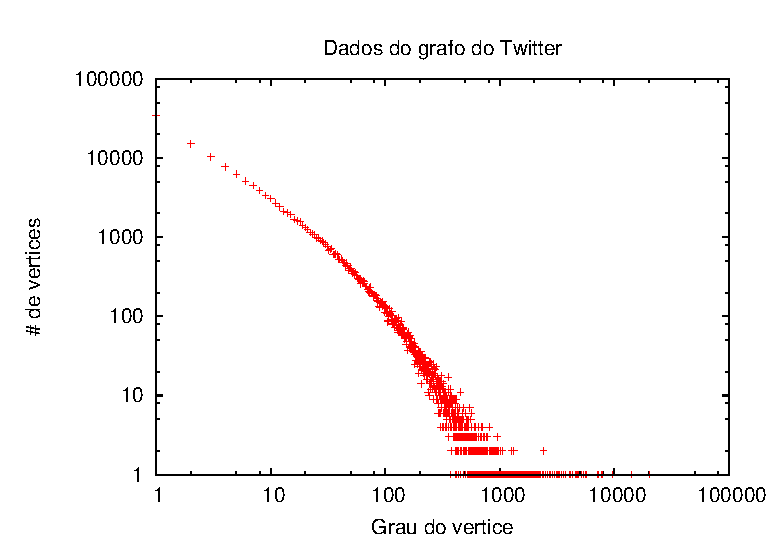
\includegraphics{power_law.eps}}
	\caption{Distribuição de dados de redes sociais (\emph{power-law}) com dados do Twitter}
	\label{fig:powerlaw}
\end{figure}

